\section{Analyse de domaine}
% \begin{frame}{Analyse de domaine}
% À partir de l'activité:
% \begin{itemize}
% \item Étude de scénarios.
% \item Définition de la sensibilité au contexte.
% \end{itemize}
% \end{frame}
\begin{frame}{Expérimentation écologique à large échelle}
\onslide<1->{
\begin{coloredbox}[black]{Domassist}
Déploiement~:
  \begin{itemize}
  \item 12 mois.
  \item 129 personnes vivant seules.
  \item 82 ans en moyenne.
  \end{itemize}

%% Avantage d'un déploiement large échelle:
 %  \begin{itemize}
 %  \item Seniors avec troubles cognitifs implique un éventail de services.
 %  \item Étude à long terme implique de la réactivité de la maintenance.
 %  \item Déploiement large échelle nécessite des services d'administration.
 %  %\item Les services déployés couvrent l'ensemble des besoins de l'assistance domiciliaire (assistance, maintenance, $\dots$)
 %  \end{itemize}
\end{coloredbox}
}
\vfill
\onslide<2->{
%\begin{coloredbox}[blue]{}
\centering
Différents services déployés (assistance, maintenance, $\dots$).
%\end{coloredbox}
}
\end{frame}

\subsection{Scénarios d'assistance}
\begin{frame}{Contextes dans l'assistance domiciliaire}
  \begin{minipage}[t]{0.45\linewidth}
    \begin{table}[!h]
      \begin{footnotesize}
        \begin{tabular}{| p{2.cm} | p{5.5cm} |} \hline
          {\bf Nom} & {\bf Description} \\ \hline \hline
          Alerte porte d'entrée & Entrance door \colorbox{black!2}{is open} \colorbox{black!2}{and}  \colorbox{black!2}{is unattended} \colorbox{black!2}{for 5 minutes} \\ \hline
          Réchauffer un plat surgelé  & Freezer \colorbox{black!2}{gets opened} \colorbox{black!2}{and} stove \colorbox{black!2}{gets turned on} \colorbox{black!2}{within 10 minutes} \colorbox{black!2}{or} Freezer \colorbox{black!2}{gets opened} \colorbox{black!2}{during} stove \colorbox{black!2}{is on}, \colorbox{black!2}{during} \colorbox{black!2}{lunch time} \\ \hline
          Dépendance de présence & The cupboard \colorbox{black!2}{gets opened} in the kitchen, \colorbox{black!2}{while} a presence in the kitchen \colorbox{black!2}{is false} \\ \hline
          Échec de communication & A sensor \colorbox{black!2}{fails to communicate} \colorbox{black!2}{for 24 hours} %and its status does not \dashuline{get updated} 
          \\ \hline
        \end{tabular}
      \end{footnotesize}
    \end{table}
  \end{minipage}
  \hfill
  \begin{minipage}[t]{0.38\linewidth}
    Commonalités~:\\
    \vspace*{20.7mm}

    Variabilités~:
  \end{minipage}
\end{frame}
\subsection{Scénarios d'assistance}
\addtocounter{framenumber}{-1}
\begin{frame}{Contextes dans l'assistance domiciliaire}
  \begin{minipage}[t]{0.45\linewidth}
    \begin{table}[!h]
      \begin{footnotesize}
        \begin{tabular}{| p{2.cm} | p{5.5cm} |} \hline
          {\bf Nom} & {\bf Description} \\ \hline \hline
          Alerte porte d'entrée & Entrance door \colorbox{black!2}{is open} \colorbox{black!2}{and}  \colorbox{black!2}{is unattended} \colorbox{black!2}{for 5 minutes} \\ \hline
          Réchauffer un plat surgelé  & Freezer \colorbox{black!2}{gets opened} \colorbox{black!2}{and} stove \colorbox{black!2}{gets turned on} \colorbox{black!2}{within 10 minutes} \colorbox{black!2}{or} Freezer \colorbox{black!2}{gets opened} \colorbox{black!2}{during} stove \colorbox{black!2}{is on}, \colorbox{black!2}{during} \colorbox{black!2}{lunch time} \\ \hline
          Dépendance de présence & The cupboard \colorbox{black!2}{gets opened} in the kitchen, \colorbox{black!2}{while} a presence in the kitchen \colorbox{black!2}{is false} \\ \hline
          Échec de communication & A sensor \colorbox{black!2}{fails to communicate} \colorbox{black!2}{for 24 hours} %and its status does not \dashuline{get updated} 
          \\ \hline
        \end{tabular}
      \end{footnotesize}
    \end{table}
  \end{minipage}
  \hfill
  \begin{minipage}[t]{0.38\linewidth}
    Commonalités~:
    \begin{itemize}
    \item Mesures d'environnement (physique et numérique).
    
    \end{itemize}
    \vspace*{13.1mm}
    Variabilités~:
  \end{minipage}
\end{frame}

\subsection{Scénarios d'assistance}
\addtocounter{framenumber}{-1}
\begin{frame}{Contextes dans l'assistance domiciliaire}
  \begin{minipage}[t]{0.45\linewidth}
    \begin{table}[!h]
      \begin{footnotesize}
        \begin{tabular}{| p{2.cm} | p{5.5cm} |} \hline
          {\bf Nom} & {\bf Description} \\ \hline \hline
          Alerte porte d'entrée & Entrance door \colorbox{black!2}{is open} \colorbox{black!2}{and}  \colorbox{black!2}{is unattended} \colorbox{black!2}{for 5 minutes} \\ \hline
          Réchauffer un plat surgelé  & Freezer \colorbox{checked!50}{gets opened} \colorbox{black!2}{and} stove \colorbox{checked!50}{gets turned on} \colorbox{black!2}{within 10 minutes} \colorbox{black!2}{or} Freezer \colorbox{checked!50}{gets opened} \colorbox{black!2}{during} stove \colorbox{black!2}{is on}, \colorbox{black!2}{during} \colorbox{black!2}{lunch time} \\ \hline
          Dépendance de présence & The cupboard \colorbox{checked!50}{gets opened} in the kitchen, \colorbox{black!2}{while} a presence in the kitchen \colorbox{black!2}{is false} \\ \hline
          Échec de communication & A sensor \colorbox{black!2}{fails to communicate} \colorbox{black!2}{for 24 hours} %and its status does not \dashuline{get updated} 
          \\ \hline
        \end{tabular}
      \end{footnotesize}
    \end{table}
  \end{minipage}
  \hfill
  \begin{minipage}[t]{0.38\linewidth}
    Commonalités~:
    \begin{itemize}
    \item Mesures d'environnement (physique et numérique).
    \item \colorbox{checked!50}{Évènements}.
    \end{itemize}
    \vspace*{6.55mm}
    Variabilités~:
  \end{minipage}
\end{frame}
\subsection{Scénarios d'assistance}
\addtocounter{framenumber}{-1}
\begin{frame}{Contextes dans l'assistance domiciliaire}
  \begin{minipage}[t]{0.45\linewidth}
    \begin{table}[!h]
      \begin{footnotesize}
        \begin{tabular}{| p{2.cm} | p{5.5cm} |} \hline
          {\bf Nom} & {\bf Description} \\ \hline \hline
          Alerte porte d'entrée & Entrance door \colorbox{darkgray!50}{is open} \colorbox{black!2}{and}  \colorbox{darkgray!50}{is unattended} \colorbox{black!2}{for 5 minutes} \\ \hline
          Réchauffer un plat surgelé  & Freezer \colorbox{checked!50}{gets opened} \colorbox{black!2}{and} stove \colorbox{checked!50}{gets turned on} \colorbox{black!2}{within 10 minutes} \colorbox{black!2}{or} Freezer \colorbox{checked!50}{gets opened} \colorbox{black!2}{during} stove \colorbox{darkgray!50}{is on}, \colorbox{black!2}{during} \colorbox{darkgray!50}{lunch time} \\ \hline
          Dépendance de présence & The cupboard \colorbox{checked!50}{gets opened} in the kitchen, \colorbox{black!2}{while} a presence in the kitchen \colorbox{darkgray!50}{is false} \\ \hline
          Échec de communication & A sensor \colorbox{darkgray!50}{fails to communicate} \colorbox{black!2}{for 24 hours} %and its status does not \dashuline{get updated} 
          \\ \hline
        \end{tabular}
      \end{footnotesize}
    \end{table}
  \end{minipage}
  \hfill
  \begin{minipage}[t]{0.38\linewidth}
    Commonalités~:
    \begin{itemize}
    \item Mesures d'environnement (physique et numérique).
    \item \colorbox{checked!50}{Évènements}.
    \item \colorbox{darkgray!50}{États}.
    \end{itemize}
    Variabilités~:
  \end{minipage}
\end{frame}


\subsection{Scénarios d'assistance}
\addtocounter{framenumber}{-1}
\begin{frame}{Contextes dans l'assistance domiciliaire}
  \begin{minipage}[t]{0.45\linewidth}
    \begin{table}[!h]
      \begin{footnotesize}
        \begin{tabular}{| p{2.cm} | p{5.5cm} |} \hline
          {\bf Nom} & {\bf Description} \\ \hline \hline
          Alerte porte d'entrée & Entrance door \colorbox{darkgray!50}{is open} \colorbox{teal!50}{and}  \colorbox{darkgray!50}{is unattended} \colorbox{teal!50}{for 5 minutes} \\ \hline
          Réchauffer un plat surgelé  & Freezer \colorbox{checked!50}{gets opened} \colorbox{teal!50}{and} stove \colorbox{checked!50}{gets turned on} \colorbox{teal!50}{within 10 minutes} \colorbox{teal!50}{or} Freezer \colorbox{checked!50}{gets opened} \colorbox{teal!50}{during} stove \colorbox{darkgray!50}{is on}, \colorbox{teal!50}{during} \colorbox{darkgray!50}{lunch time} \\ \hline
          Dépendance de présence & The cupboard \colorbox{checked!50}{gets opened} in the kitchen, \colorbox{teal!50}{while} a presence in the kitchen \colorbox{darkgray!50}{is false} \\ \hline
          Échec de communication & A sensor \colorbox{darkgray!50}{fails to communicate} \colorbox{teal!50}{for 24 hours} %and its status does not \dashuline{get updated} 
          \\ \hline
        \end{tabular}
      \end{footnotesize}
    \end{table}
  \end{minipage}
  \hfill
  \begin{minipage}[t]{0.38\linewidth}
    Commonalités:
    \begin{itemize}
    \item Mesures d'environnement (physique et numérique).
    \item \colorbox{checked!50}{Évènements}.
    \item \colorbox{darkgray!50}{États}.
    \end{itemize}
    Variabilités:
    \begin{itemize}%[<+->]
    \item \colorbox{teal!50}{Contraintes d'interactions} (précédence, chevauchement, durée,$~\dots$).
    %\item Niveaux d'abstraction.
    \end{itemize}
  \end{minipage}
\end{frame}


\begin{frame}{Concepts spécifiques au domaine}
\onslide<1->{
\begin{minipage}{.45\linewidth}
\begin{coloredbox}[checked]{Évènement}
\footnotesize
Changement de valeur pour \\une entité mesurée, à un instant donné.
\end{coloredbox}
\end{minipage}
\hfill
\begin{minipage}{.45\linewidth}
\begin{coloredbox}[darkgray]{État}
\footnotesize
Valeur persistante durant une période. \\Commence à un instant donné, \\termine à un instant donné.
\end{coloredbox}
\end{minipage}
}
  % \begin{itemize}
  % \item\colorbox{checked!10}{Évènement}~: changement de valeur pour une entité mesurée, à un instant donné
  % \item \colorbox{blue!5}{États}~: valeur persistante durant une période. Commence à un instant donné, termine à un instant donné.
  % \end{itemize}
\vfill
\onslide<2->{
\begin{coloredbox}[red]{Besoins communs}
  \begin{itemize}
  \item Couvrir les différents objectifs.
  \item Couvrir l'hétérogénéité des données.
  \item Récurrences des interactions dans le flux d'évènements.
  \item Expressivité temporelle adaptée au domaine.
  \item Réactivité des services.
  \end{itemize}
\end{coloredbox}
}
% Besoins communs:
%   \begin{itemize}
%   \item Réactivité des services.
%   \item Couvrir les différents objectifs.
%   \item Couvrir l'hétérogénéité des données.
%   \item Récurrences des interactions dans le flux d'évènements.
%   \item Expressivité temporelle.
%   \end{itemize}
\end{frame}

\subsection{Définition de la sensibilité au contexte}
\begin{frame}{Implantation domiciliaire du contexte}
  \begin{minipage}{.48\linewidth}
    \begin{coloredbox}[black]{}
      \begin{scriptsize}
        Freezer gets opened and stove gets turned on within 10 minutes during lunch time.
      \end{scriptsize}
    \end{coloredbox}
  \end{minipage}
  \hfill
  \begin{minipage}{.48\linewidth}
    % \begin{scriptsize}
    %   a presence in the Bedroom is true and a presence in the Kitchen is true within 10 minutes
    % \end{scriptsize}
  \end{minipage}
  \vfill
  \begin{minipage}{0.45\linewidth}
    \begin{coloredbox}[teal]{Préparation du déjeuner}
\small
    \begin{itemize}
    \item Ouvrir la porte du congélateur.
      \begin{itemize}
      \item 
\includegraphics[scale=0.2]{csensor.png} Capteur de contact
      \end{itemize}
    \item Allumer le four.
      \begin{itemize}
      \item 
\includegraphics[scale=0.2]{emeter.png} Capteur de consommation électrique.
      \end{itemize}
    \end{itemize}
\end{coloredbox}
  \end{minipage}
  \hfill
  \begin{minipage}{0.50\linewidth}
    \begin{figure}
      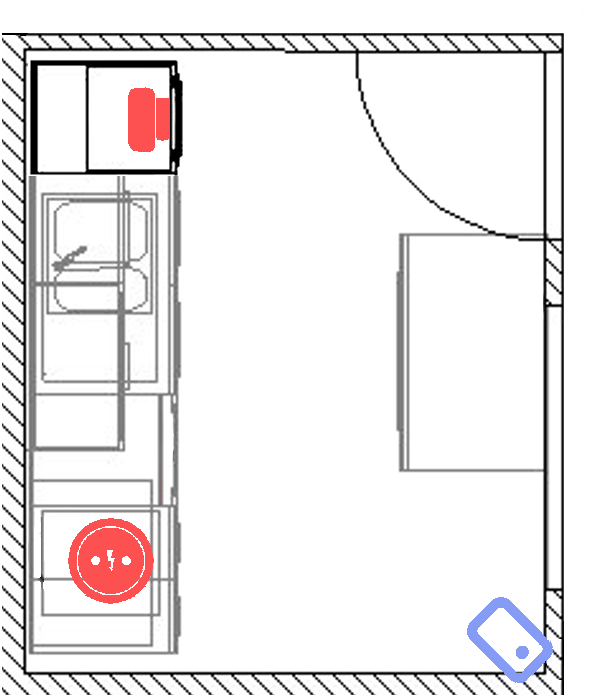
\includegraphics[scale=0.20]{use_case1.png}
    \end{figure}
  \end{minipage}
\end{frame}
% **********************************************
\begin{frame}{Implantation domiciliaire du contexte}
  \addtocounter{framenumber}{-1}
\begin{minipage}{.48\linewidth}
    \begin{coloredbox}[black]{}
      \begin{scriptsize}
        Freezer gets opened and stove gets turned on within 10 minutes during lunch time.
      \end{scriptsize}
    \end{coloredbox}
  \end{minipage}
  \hfill
  \begin{minipage}{.48\linewidth}
    % \begin{scriptsize}
    %   a presence in the Bedroom is true and a presence in the Kitchen is true within 10 minutes
    % \end{scriptsize}
  \end{minipage}
  \vfill
  \begin{minipage}{0.45\linewidth}
    \begin{coloredbox}[teal]{Préparation du déjeuner}
\small
    \begin{itemize}
    \item Ouvrir la porte du congélateur.
      \begin{itemize}
      \item 
\includegraphics[scale=0.2]{csensor.png} Capteur de contact
      \end{itemize}
    \item Allumer le four.
      \begin{itemize}
      \item 
\includegraphics[scale=0.2]{emeter.png} Capteur de consommation électrique.
      \end{itemize}
    \end{itemize}
\end{coloredbox}
  \end{minipage}
  \hfill
  \begin{minipage}{0.50\linewidth}
    \begin{figure}
      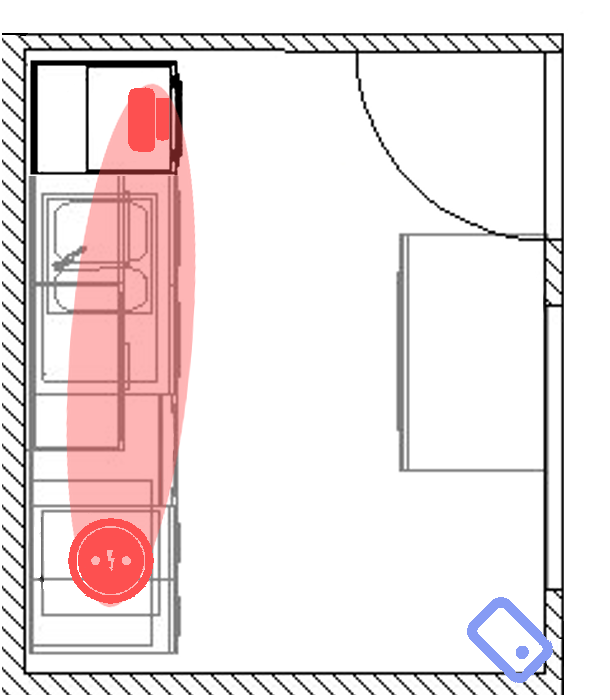
\includegraphics[scale=0.2]{use_case1_5.png}
    \end{figure}
  \end{minipage}
\end{frame}
% **********************************************
\begin{frame}{Implantation domiciliaire du contexte}
  \addtocounter{framenumber}{-1}
  \begin{minipage}{.48\linewidth}
    % \begin{coloredbox}[black]{}
    %   \begin{scriptsize}
    %     Freezer gets opened and stove gets turned on within 10 minutes during lunch time
    %   \end{scriptsize}
    % \end{coloredbox}
  \end{minipage}
  \hfill
  \begin{minipage}{.48\linewidth}
    % \vspace*{2.7mm}
    \begin{coloredbox}[black]{}
      \begin{scriptsize}
        A presence in the Bedroom is true then\\ a presence in the Kitchen is true.% within 10 minutes
      \end{scriptsize}
    \end{coloredbox}
  \end{minipage}
  \vfill

  \begin{minipage}{0.45\linewidth}
    \begin{coloredbox}[teal]{Lever}
      \small
      \begin{itemize}
      \item Présence dans la cuisine.
        \begin{itemize}
        \item 
\includegraphics[scale=0.2]{mdetect.png} Capteur de mouvement
        \end{itemize}
        % \item Allumer le four.
        %   \begin{itemize}
        %   \item 
\includegraphics[scale=0.2]{emeter.png} Capteur de consommation électrique.
        %   \end{itemize}
      \end{itemize}
    \end{coloredbox}
  \end{minipage}
  \hfill
  \begin{minipage}{0.50\linewidth}
    \begin{figure}
      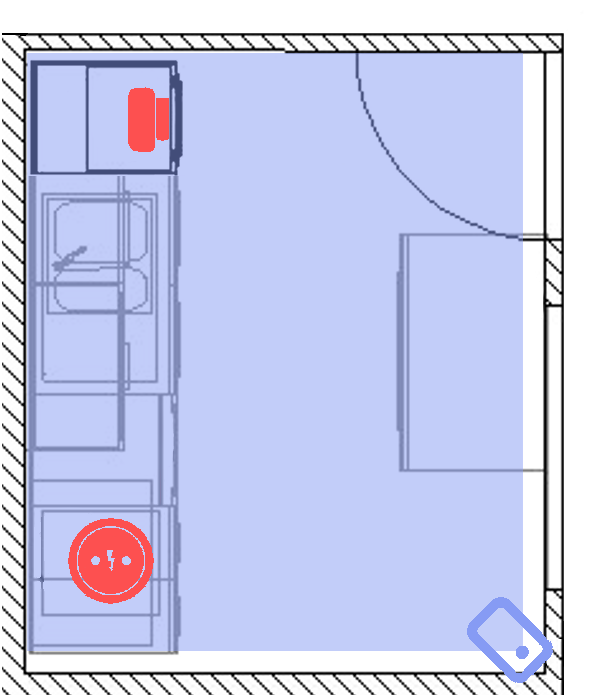
\includegraphics[scale=0.2]{use_case1_2.png}
    \end{figure}
  \end{minipage}
\end{frame}
% **********************************************
\begin{frame}{Implantation domiciliaire du contexte}
  \addtocounter{framenumber}{-1}
\begin{minipage}{.48\linewidth}
    \begin{coloredbox}[black]{}
      \begin{scriptsize}
        Freezer gets opened and stove gets turned on within 10 minutes during lunch time.
      \end{scriptsize}
    \end{coloredbox}
  \end{minipage}
  \hfill
  \begin{minipage}{.48\linewidth}
    \begin{coloredbox}[black]{}
      \begin{scriptsize}
        A presence in the Bedroom is true then\\ a presence in the Kitchen is true.% within 10 minutes
      \end{scriptsize}
    \end{coloredbox}
  \end{minipage}
  \vfill

  \begin{minipage}{0.45\linewidth}
\begin{coloredbox}[teal]{Modèle implicite}
    %Modèle implicite~:
\small
    \begin{itemize}
    \item Détection de mouvement précède toute autre interaction.
    \item Une présence dans une pièce ne peut pas recouvrir une présence dans une autre pièce.
    \end{itemize}
\end{coloredbox}
  \end{minipage}
  \hfill
  \begin{minipage}{0.50\linewidth}
    \begin{figure}
      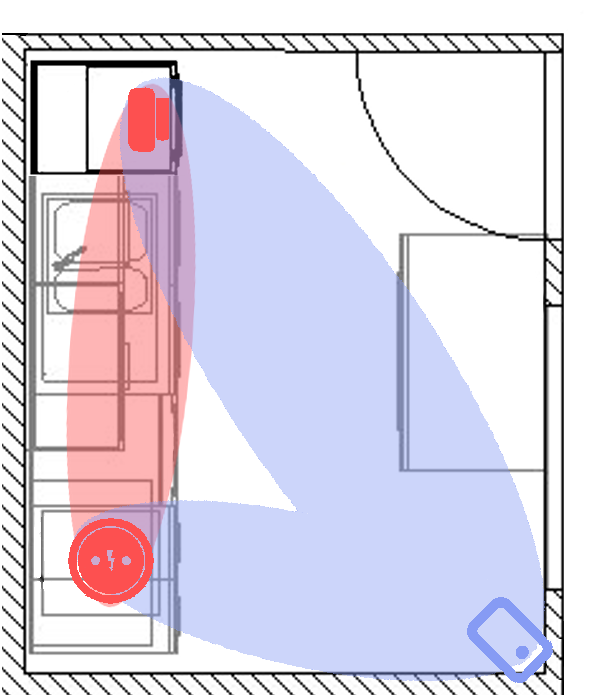
\includegraphics[scale=0.2]{use_case2.png}
    \end{figure}
  \end{minipage}
\end{frame}

% **********************************************


\subsection{Synthèse}
\begin{frame}{Synthèse}
  \begin{minipage}[t]{0.3\linewidth}
    \begin{figure}
      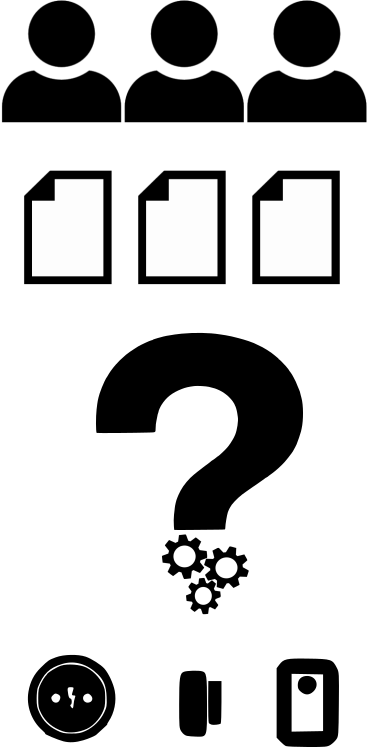
\includegraphics[scale=0.3]{synthese_domain.png}
    \end{figure}
  \end{minipage}
  \begin{minipage}[t]{0.68\linewidth}
    %Besoins:
    \begin{itemize}
      \item Concepts spécifiques au domaine.
      \item Expressivité des services.
    \end{itemize}
    \begin{questionbox}
      Comment couvrir les besoins \\d'expressivité de services sensibles au contexte?
    \end{questionbox}
    \vfill
    \begin{itemize}
      \item Implantation de la sensibilité au contexte.
      \item Modèle implicite.%Fiabilité de la sensibilité au contexte.
    \end{itemize}
    \begin{questionbox}
      Comment rendre explicite le modèle implicite, basé sur les hypothèses?
    \end{questionbox}
  \end{minipage}
\end{frame}